\documentclass[10pt,
			   xcolor=svgnames,
			   hyperref={linkcolor=red, citecolor = DarkGreen, colorlinks=true, urlcolor=Navy}]{beamer}
			   
\usepackage[english]{babel}
\usepackage[utf8x]{inputenc}

\usepackage{tikz}
\def\checkmark{\tikz\fill[scale=0.4](0,.35) -- (.25,0) -- (1,.7) -- (.25,.15) -- cycle;}

\mode<presentation>
{
  \usetheme{Copenhagen}      % or try Darmstadt, Madrid, Warsaw, ...
  \usecolortheme{beaver}
} 

\usepackage{multicol}
\setlength{\columnseprule}{0.pt}

\usepackage{float}
\usepackage[authoryear]{natbib}

\graphicspath{{./pic/}}

\usepackage[font=scriptsize, center]{caption}

%%% Commandes utiles définies
\newcommand{\argmin}{\mathop{\mathrm{argmin}}}

\newcommand{\bepar}[1]{
	\left( #1 \right)  
}
\newcommand{\becro}[1]{
	\left[ #1 \right]  
}

\xdefinecolor{bviolet}{named}{BlueViolet}

%%%%%%%%%%%%%%%%%%%%
%%% Couleurs %%%
\xdefinecolor{brick}{named}{DarkRed}
\xdefinecolor{navy}{named}{Navy}
\xdefinecolor{midblue}{named}{MidnightBlue}
\xdefinecolor{dsb}{named}{DarkSlateGray}
\xdefinecolor{dgreen}{named}{DarkGreen}

%%% 	Raccourcis 	%%%
\newcommand{\keps}{$k-\varepsilon$}
\newcommand\bk{\color{black}}
\newcommand\brick{\color{brick}}
\newcommand\navy{\color{navy}}
\newcommand\midblue{\color{midblue}}
\newcommand\dsb{\color{dsb}}
\newcommand{\dgreen}{\color{dgreen}}
\newcommand\red{\color{red}}


% Things for first slide :
\title[Machine learning in Physics fields]{An attempt to learn Physics : ML in fluid mechanics problems}
\author{Saura Nathaniel\\}
\institute{\bf LMFL}
\date{$5^{\text{th}}$ July 2018}

% Begin 
\begin{document}
\begin{frame}
  \titlepage
\end{frame}

\begin{frame}{Main idea through few observations}

\begin{block}{Well known question : cost computation or precision ?}
\begin{itemize}
\item[$\bullet$] DNS provides perfect solutions but needs a lot of time computation
\item[$\bullet$] RANS models provide quicker more or less precise results 
\end{itemize} 
\end{block}
\vspace{1cm}
\begin{block}{ML algorithms exploding development (in every field)}
\begin{itemize}
\item[$\bullet$] Gaussian Process
\item[$\bullet$] RForests, NNetworks (Supervised) for classification or regression tasks (more and more papers in Physics field)
\item[$\bullet$] Reinforcement Learning (Semi-Supervised) (few papers)
\end{itemize}
\end{block}

\end{frame}

\begin{frame}{Main idea through few observations}
\begin{block}{Different implementations}
\begin{itemize}
	\item[$\bullet$] Data-Driven augmentation (use of high fidelity datasets) with a combination of Bayesian Inference and Gaussian Process (or other ML methods)
	\item[$\bullet$] Machine Learning to whole recover physical behaviour
\end{itemize}
\end{block} 

\tableofcontents

\end{frame}

\section{Bayesian inversion framework (BIF)}
\begin{frame}{Infer beta through inversion}
\begin{block}{Modified closure equation }
The main idea of RANS models is to add a closure equation. The main idea of BI is to add a flexible term in this closure to correct the error injected.  
\center{$\displaystyle \mathcal{F}\bepar{\color{BlueViolet} \beta(\mathbf{x}, t) \bk P_{\text{roduction}}  - D_{\text{issipation} } + T_{\text{ransport}}} = 0 $}
\end{block}
$$ \beta_M = \argmin \mathcal{J}$$
$$\mathcal{J} = \becro{\frac{1}{2} \bepar{\text{Obs} - h\bepar{\beta}}^T\textbf{C}^{-1}_m\bepar{\text{Obs} - h\bepar{\beta}} + \bepar{\beta - \beta_{\text{p}}}^T\textbf{C}_\beta^{-1}\bepar{\beta - \beta_{\text{p}}}}$$

\begin{block}{Importance and meaning of $\beta$}
\begin{itemize}
\item[$\bullet$] Discrepancy vector minimizing the distance between DNS and RANS solutions (can be seen as a vector of latent variables)
\item[$\bullet$] Maximizing $\color{BlueViolet} \beta \bk | \text{Obs}$ 
\end{itemize}
\end{block}

\end{frame}
\begin{frame}{Bayesian Inversion Framework (BIF)}
Framework proposed by Duraisamy \textit{et. al} in \citep{parish2016paradigm}
\begin{multicols*}{2}
\noindent
	\begin{figure}[!ht]
	\centering
	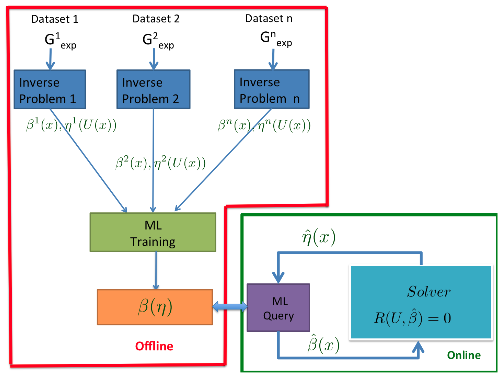
\includegraphics[scale=0.3]{singh.png}
	\caption{Figure extracted from \citep{singh2017machine}}
	\end{figure}
	
	\columnbreak

	\begin{itemize}
	\item[1 --] Infer descrepancy \color{BlueViolet} \textit{information} \bk $\beta$ as the MAP solution \\[5mm]
	
	\item[2 --]	\textit{Generalize} this information using ML methods to have a \color{BlueViolet} \textit{knowledge} \bk: $\beta = \mathcal{F}\bepar{\eta_1, \eta_2,...}$ \\[5mm]
 
	\item[3 --] Inject ML predicted correction into model's equation(s) \\[5mm]
	
	\end{itemize}
			
\end{multicols*}
\end{frame}

\begin{frame}{BIF example : 1D heat conduction with radiative and conductive heat sources}
\begin{block}{Real and Model equations}
\begin{itemize}
\item[$\bullet$] Real equation :
\begin{center}
$\displaystyle \frac{d^2T}{dz^2} + \varepsilon(T)\bepar{T^4_\infty - T^4} + h\bepar{T_\infty - T} = 0$
\end{center}
\item[$\bullet$] Model equation :
\begin{center}
$\displaystyle \frac{d^2T}{dz^2} + \varepsilon_0\color{BlueViolet}\beta(z)\bk\bepar{T^4_\infty - T^4}= 0$
\end{center}
\end{itemize} 
\end{block}

\begin{itemize}
\item[\dgreen \checkmark] BFGS method to minimize $\mathcal{J}$ $\rightarrow$ $\beta_{\text{MAP}}$ \& $\text{Hess}^{-1}_{\beta_{\text{MAP}}}$
\item[\dgreen \checkmark] Create $\beta_{\text{final}}$ distribution : \\
\begin{center}
$ \beta_{\text{final}} = \beta_M + \text{Chol}\bepar{{\text{Hess}^{-1}_{\beta_{\text{MAP}}}}}\cdot\ \text{s}$
\end{center}
$\rightarrow s \sim \mathcal{N}\bepar{0, 1},\ \text{and}\ \beta_{\text{final}} \equiv \beta \sim \mathcal{N}\bepar{\beta_{\text{MAP}}, {\text{Hess}^{-1}_{\beta_{\text{MAP}}}}}$
\end{itemize}

\end{frame}

\begin{frame}{BIF : Few figures based on inversion ($T_\infty = 15$C)}
\begin{multicols}{2}
\noindent
	\begin{figure}[H]
	\centering
	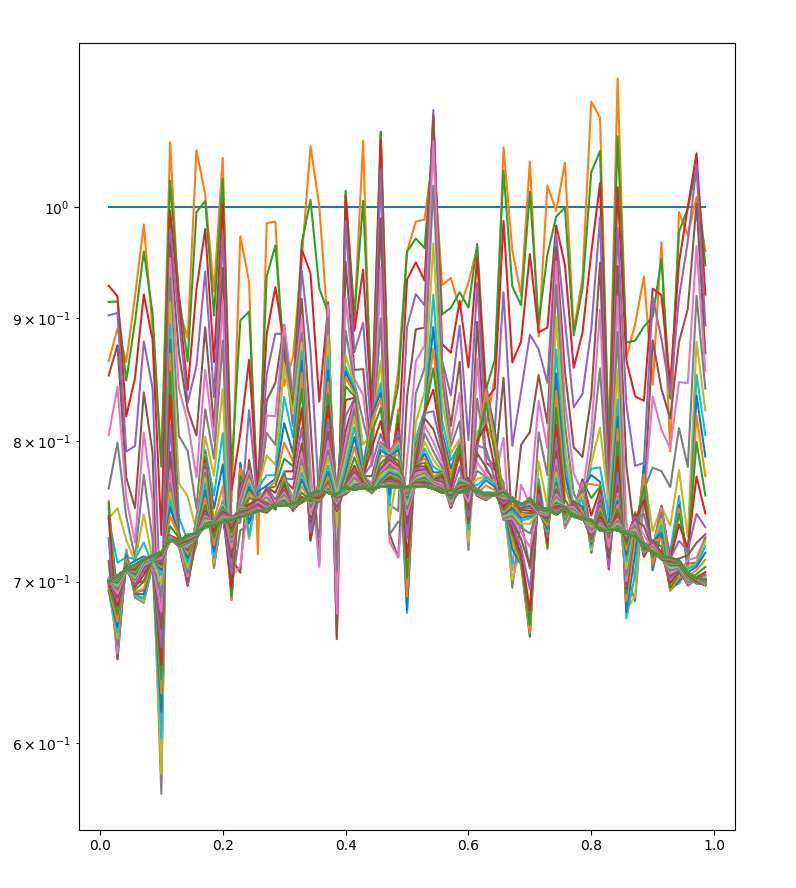
\includegraphics[scale=0.2]{Pres_Evolution_beta_map.png}
	\end{figure}

\columnbreak
	
	\vspace*{-1cm}
	\begin{figure}[H]
	\centering
	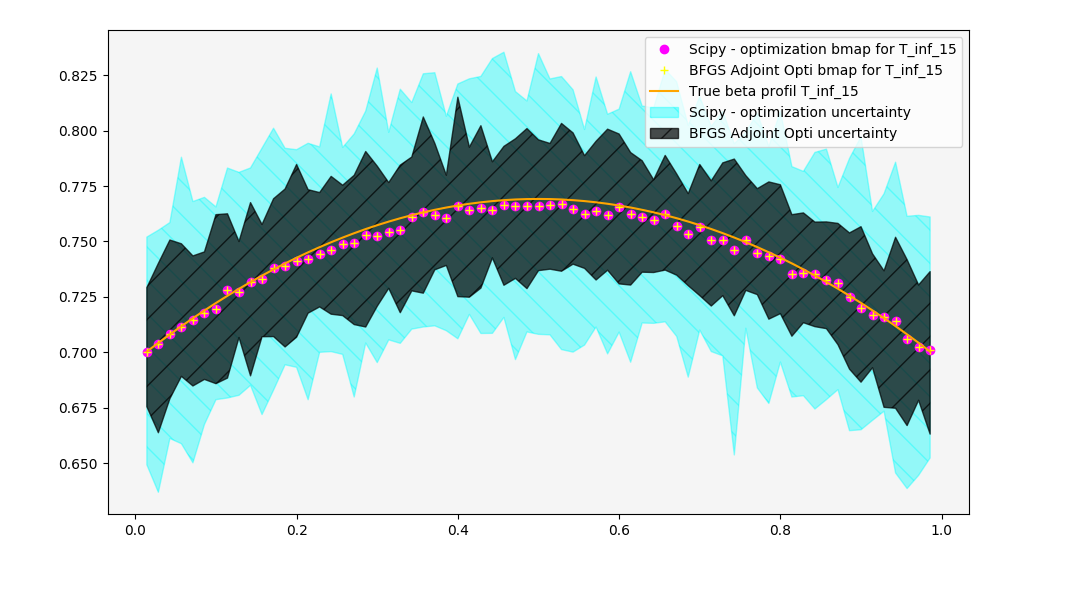
\includegraphics[height=4cm, width=6cm]{Pres_T_15_Full_Beta_Comp.png}
	\end{figure}
	
	\vspace*{-2cm}
	\begin{figure}[H]
	\centering
	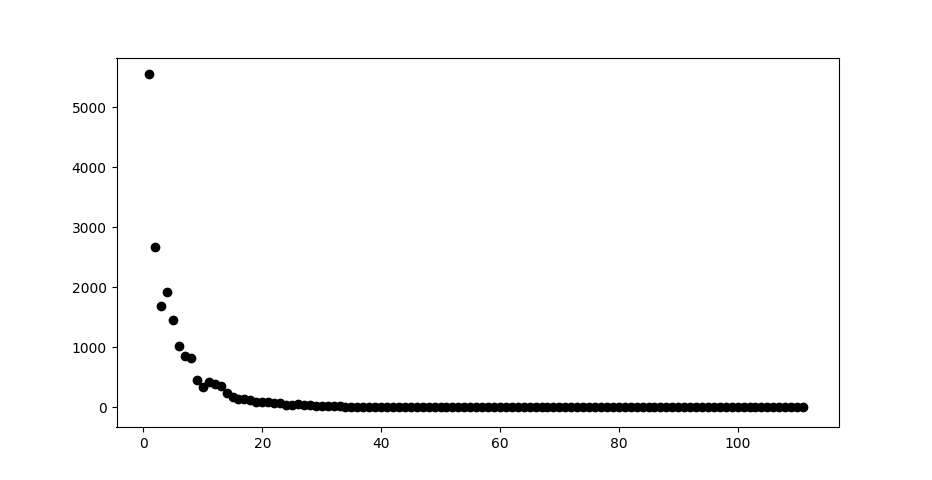
\includegraphics[height=4cm, width=6cm]{Pres_Evolution_de_l'erreur_T_inf_15.png}
	\end{figure}		


	
\end{multicols}
\end{frame}

\begin{frame}{BIF : Next Step : Machine Learning}
Reproduce the previous calculs for T = 5:5:50 \\[1cm]

Construction $X$ and $y$ in $\mathcal{D} = \left\lbrace \ \underbrace{\bepar{T_{\text{inf}},T(x_i)}}_{X_i}, \ \underbrace{\beta_i}_{y_i}\ \right\rbrace$ for each T.\\
In matrix notation : 

\begin{multicols}{2}
\noindent
$$ X = \left[ \begin{array}{c} \cdot \\ \cdot \\ T_{\text{inf}},\ T(x) \\ \cdot \\ \cdot
			  \end{array}
	   \right]
$$
\columnbreak
$$ y = \left[ \begin{array}{c} \cdot \\ \cdot \\ \beta(x) \\ \cdot \\ \cdot
			  \end{array}
	   \right]
$$
\end{multicols}
Neural Network generalizes $\beta_1, \beta_2, ..., \beta_n \rightarrow \beta_{\text{ML}} = \mathcal{F}\bepar{T_{\text{inf}}, T}$
\end{frame}

\begin{frame}
\bibliographystyle{apalike}
\bibliography{bibliotheque}
\end{frame}

\end{document}